\documentclass[conference]{IEEEtran}
\IEEEoverridecommandlockouts
% The preceding line is only needed to identify funding in the first footnote. If that is unneeded, please comment it out.
%Template version as of 6/27/2024

% Türkçe karakterler için gerekli paketler
\usepackage[utf8]{inputenc}
\usepackage[T1]{fontenc}
\usepackage{turkish}

\usepackage{cite}
\usepackage{amsmath,amssymb,amsfonts}
\usepackage{algorithmic}
\usepackage{graphicx}
\usepackage{textcomp}
\usepackage{xcolor}
\usepackage{url}
\def\BibTeX{{\rm B\kern-.05em{\sc i\kern-.025em b}\kern-.08em
    T\kern-.1667em\lower.7ex\hbox{E}\kern-.125emX}}
\begin{document}

\title{Çözebilir mi?}

\author{\IEEEauthorblockN{Eyüp Dalan}
\IEEEauthorblockA{\textit{Fen Bilimleri Enstitüsü - Bilgisayar Mühendisliği} \\
\textit{Yıldız Teknik Üniversitesi}\\
İstanbul, Türkiye \\
eyupdalan@gmail.com}
}

\maketitle

\begin{abstract}
Bu çalışmada, ortaokul seviyesi matematik problemlerini çözme performansı embedding-tabanlı sınıflandırma yöntemleriyle analiz edilmiştir. GSM8K-TR veri seti kullanılarak, farklı dil modellerinin performansları karşılaştırılmış ve sınıflandırma doğruluğu değerlendirilmiştir.
\end{abstract}

\begin{IEEEkeywords}
matematik problemi, embedding, sınıflandırma, dil modelleri, performans analizi
\end{IEEEkeywords}

\section{Giriş}

Bu çalışmada elimizdeki ortaokul seviyesi matematik problem ve cevaplarını içeren veri seti kullanılarak, farklı modellerin cevaplama performansları, embedding-tabanlı sınıflayıcılar ile anlamlı bir doğrulukla tahmin edebilir mi konusu incelenecektir.

Kullanılan veri setinde (GSM8K-TR)~\footnote{\url{https://huggingface.co/datasets/ytu-ce-cosmos/gsm8k_tr}} sadece soru ve cevaplar yer almaktadır. İlk olarak Open AI'ın GPT-4o modeli kullanılarak bu soru tipleri ve cevap yöntemleri tespit edilmiş, sonrasında bu veri setinin, yüksek doğruluklu Turkish-e5-large embedding modeli ile, embedding'leri çıkarılmıştır. Sonrasında da Turkish-Llama-8b-DPO-v0.1 ve Gemma-2-9b-it modellerinin bu soruları cevaplaması sağlanmış, mevcuttaki cevap ile karşılaştırılarak cevabın doğru olup olmadığı etiketlenmiştir. Son olarak, lojistik regresyon ve t-SNE görselleştirmesi kullanarak embedding uzayında sınıflandırma performansı ölçülmüş ve sonuçları karşılaştırılmıştır. 

\section{Yöntem}
Bu bölümde, çalışma akışındaki adımlar ayrıntılı olarak açıklanmaktadır.

\subsection{Kullanılan Veri Seti}
GSM8K-TR veri seti kullanılmıştır. Bu veri seti aşağıdaki özellikleri içerir:
\begin{itemize}
\item İki temel sütun: "question" (soru) ve "answer" (cevap).
\item Toplam 8792 kayıt.
\end{itemize}

\subsection{Model Çözümleri ve Etiketleme}
Soru çözme performanslarını değerlendirmek için aşağıdaki iki model kullanılmıştır:

\begin{itemize}
\item Turkish-Llama-8b-DPO-v0.1~\footnote{\url{https://huggingface.co/ytu-ce-cosmos/Turkish-Llama-8b-DPO-v0.1}}.
\item Gemma-2-9b-it~\footnote{\url{https://huggingface.co/google/gemma-2-9b-it}}.
\end{itemize}

Her iki model de ayrı ayrı yüklenmiş, sonra her bir soru için aşağıdaki prompt ile modelden sonuçlar alınmıştır. Burada matematiksel notasyonlardan kaçınması, açıklamadan doğrudan sonucu vermesi istenmiştir. Gelen sonuçlar her model için ayrı ayrı kaydedilmiştir.

\begin{verbatim}
prompt = (
 f"Soru: {question}"
 "Soruya tek bir yanıt ver,"
 "adım adım çözme, sadece sonuç olsun."
 "Yanıtlarında '24 × \\frac' gibi "
 "notasyonlar kullanma."
 "Sonuç: <değer> formatında göster."
)
\end{verbatim}

Tüm çıktılar elde edildikten sonra, modellerden gelen cevaplardan son sayı çıkarılarak gerçek cevapla karşılaştırılmış, eşleşme durumunda 1 (başarılı), aksi halde 0 (başarısız) etiketi atanmıştır. Elde edilen başarı sayıları:
\begin{itemize}
\item Llama Doğru: 1001, Yanlış: 7791
\item Gemma Doğru: 1558, Yanlış: 7234
\end{itemize}

Elde edilen bu çıktılarla veri seti genişletilmiştir: question, answer, tr\_llama\_result, is\_tr\_llama\_correct, gg\_gemma\_result, is\_gg\_gemma\_correct

\subsection{Soru Tipi ve Çözüm Yöntemi Tepiti}
Soru türü ve çözüm yöntemi bilgileri GPT-4o modeli kullanılarak üretilmiştir. Bunun için aşağıdaki promptlar kullanılmıştır:
\paragraph{Soru Türü Tespiti}
\begin{verbatim}
prompt = f"""
Aşağıdaki matematik sorusunun 
hangi türde olduğunu belirle.
Soru: {question}

Türü belirle ve kısa bir açıklama yaz.
Format: 
{"type": "tür", "explanation": "açıklama"}
"""
\end{verbatim}

\begin{figure}[htbp]
\centering
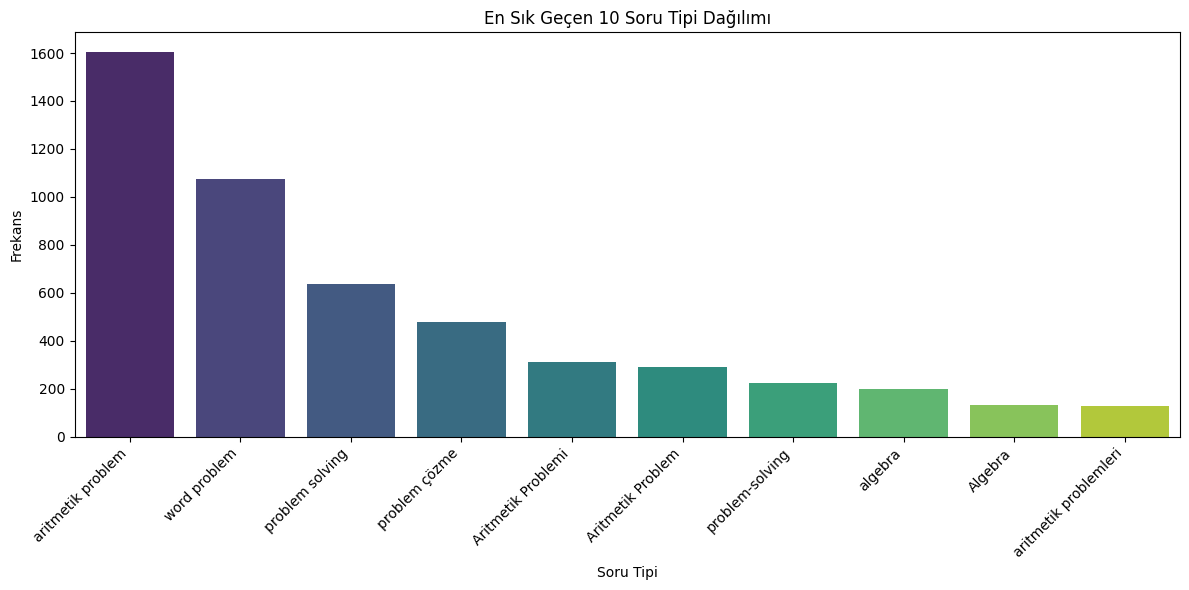
\includegraphics[width=1\linewidth]{soru-tipi.png}
\caption{En sık geçen 10 soru tipi}
\label{fig}
\end{figure}

\paragraph{Çözüm Yöntemi Tespiti}
\begin{verbatim}
prompt = f"""
Aşağıdaki matematik sorusunun cevabının 
hangi yöntemle elde edildiğini belirle.
Cevap: {answer}

Yöntemi belirle ve kısa bir açıklama yaz.
Format: 
{"method": "yöntem", "explanation": "açıklama"}
"""
\end{verbatim}

\begin{figure}[htbp]
\centering
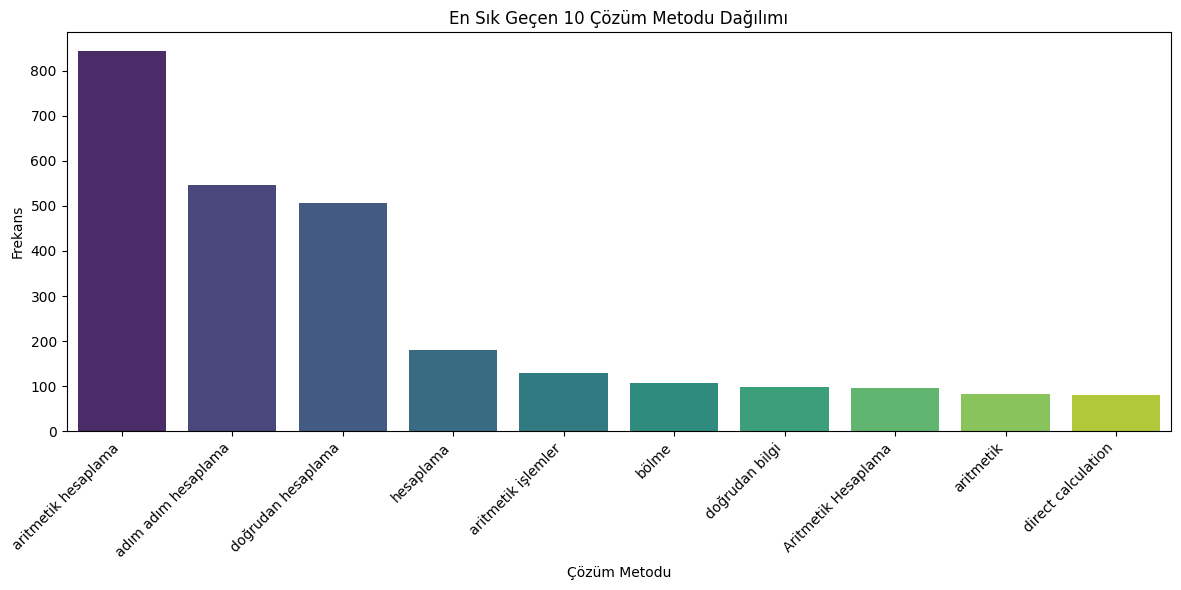
\includegraphics[width=1\linewidth]{cozum-metodu.png}
\caption{En sık geçen 10 çözüm metodu}
\label{fig}
\end{figure}

Elde edilen bu yeni kolonlarla veri seti genişletilmiştir: question, answer, tr\_llama\_result, is\_tr\_llama\_correct, gg\_gemma\_result, is\_gg\_gemma\_correct, question\_type, solution\_method.

\subsection{Embedding Çıkarımı}
Embedding'lerin çıkarımı için "ytu-ce-cosmos/turkish-e5-large"~\footnote{\url{https://huggingface.co/ytu-ce-cosmos/turkish-e5-large}} modeli kullanılmıştır. Veri setindeki aşağıdaki 4 metin kolonu için embeddingler oluşturulmuş, yine aynı veri seti genişletilerek kaydedilmiştir:

\begin{itemize}
\item question
\item answer
\item question\_type
\item solution\_method
\end{itemize}

\subsection{Lojistik Regresyon}
Soru tiplerinin ve çözüm yöntemlerinin tespitinden sonra dört adet metin verisi oluşmuş oluyor. İki modelden de çözüp çözemediğine dair sınıflandırma verisi mevcut. Bu aşamadan sonra her bir metin embedding'i için, lojistik regresyon sonucu ilgili modelin sonucunun tahminleri incelenecektir.

Elimizdeki veri seti \%50 eğitim \%50 test olarak ikiye ayrılmıştır. Sonrasında metin embedding'leri kullanılarak TR-Llama'nın ve Google Gemma'nın ayrı ayrı sınıflandırmaları karşılaştırıldı.

\begin{figure}[htbp]
\centering
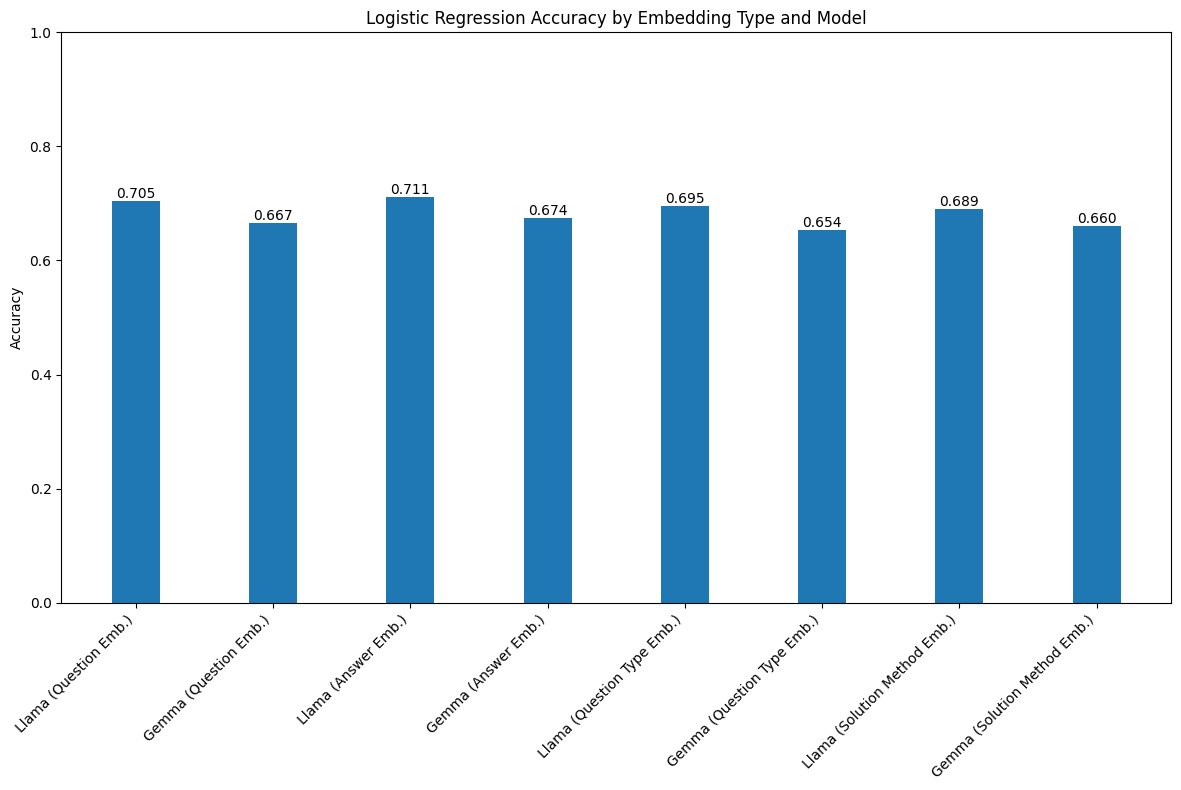
\includegraphics[width=1\linewidth]{accuracy.png}
\caption{Embedding Tipi ve Modele Göre Lojistik Regresyon Doğrulukları}
\label{fig}
\end{figure}

\section{Değerlendirme ve Tartışma}
Bu bölümde, Llama ve Gemma modellerinin dört alt görevde elde ettiği performans metrikleri ayrıntılı olarak incelenmektedir. Tablo1 ve Tablo2'de sunulan accuracy, precision, recall ve F1-score değerlerine dayanarak aşağıdaki bulgular elde edilmiştir.

\subsection{Genel Doğruluk (Accuracy) Karşılaştırması}
Llama modeli, soru çözme (\%70,50), cevap üretme (\%71,09), soru türü belirleme (\%69,47) ve çözüm yöntemi tespiti (\%68,95) görevlerinde Gemma modeline (\%66,65; \%67,45; \%65,38; \%66,04) göre 2–4 puan daha yüksek doğruluk göstermiştir. Ancak bu yüksek doğruluk oranlarının, veri setindeki \%88–\%91 oranındaki başarısız etiketler (0 sınıfı) nedeniyle bir önyargı oluşturabileceği göz önünde bulundurulmalıdır.

\subsection{Dengesiz Sınıf Dağılımının Etkisi}
Her dört görevde de 0 sınıfının destek (support) değeri 3905 iken 1 sınıfının destek değeri 491 (soru/cevap) veya 770 (soru türü/çözüm yöntemi) olarak gerçekleşmiştir. Bu dengesiz dağılım, macro ortalama F1-skorlarının (0,50–0,55) düşük kalmasına yol açmıştır.

\subsection{Minority (1) Sınıf Performansı}
1 sınıfı altında Llama modelinin precision değerleri 0,14–0,15, recall değerleri 0,33–0,40 aralığında ve F1-skorları 0,20–0,22 civarındadır. Gemma modelinde ise precision 0,24–0,25, recall 0,45–0,46 ve F1-skorları 0,31–0,32 seviyesinde görülmüştür. Bu sonuçlar, modellerin başarısızlık durumlarını (1) başarılı durumlara (0) kıyasla ayırt etmede zorlandığını göstermektedir.

\subsection{Görevlere Göre Analiz}
\textbf{Soru ve Cevap Görevleri:} Her iki modelin soru ve cevap metinleri üzerinden gerçekleştirdiği ikili sınıflandırma sonuçları benzer kalıplar sergilemiştir. Bu durum, her iki alt görevin model için eşit derecede güçlük seviyesi sunduğunu işaret eder.

\textbf{Soru Türü ve Çözüm Yöntemi:} Bu alt görevlerde de Llama modelinin Gemma'ya göre daha dengeli (yüksek doğruluk ve weighted avg F1) sonuç verdiği, ancak her iki modelin de sınıf 1'i yakalamada yetersiz kaldığı görülmüştür.

\subsection{İyileştirme Önerileri}
\begin{itemize}
\item \textbf{Veri Dengesizliği:} Az olan örneklerin çoğaltılması, modelin 1 sınıfını daha iyi öğrenmesine yardımcı olabilir.
\item \textbf{Prompt ve Etiketleme Stratejisi:} "Sonuç:" formatı yerine ek doğrulama adımları veya toleranslı eşik değerleri kullanılarak karar mekanizması geliştirilebilir.
\item \textbf{Ek Özellik Mühendisliği:} Soru uzunluğu, operatör sayısı gibi ek metin tabanlı özniteliklerin embedding ile birlikte kullanılması önerilir.
\end{itemize}

\begin{figure}[htbp]
\centering
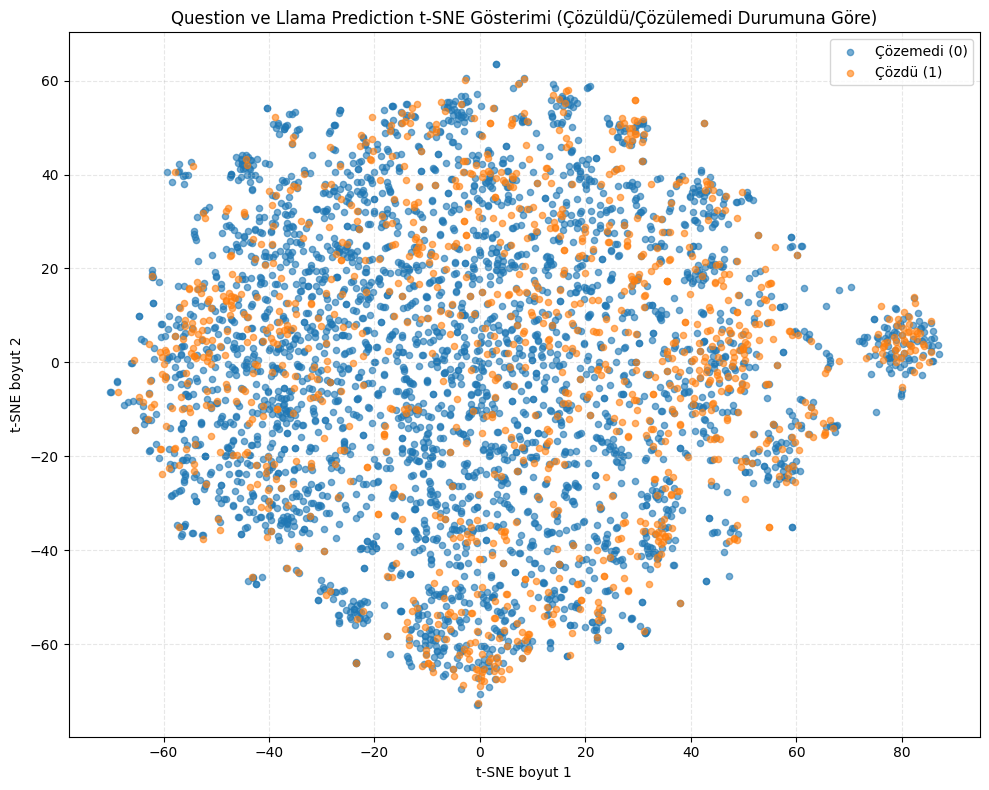
\includegraphics[width=1\linewidth]{q-l.png}
\caption{Sorular embedding'i kullanılarak yapılan TR-LLaMa tahminleri}
\label{fig}
\end{figure}

\begin{figure}[htbp]
\centering
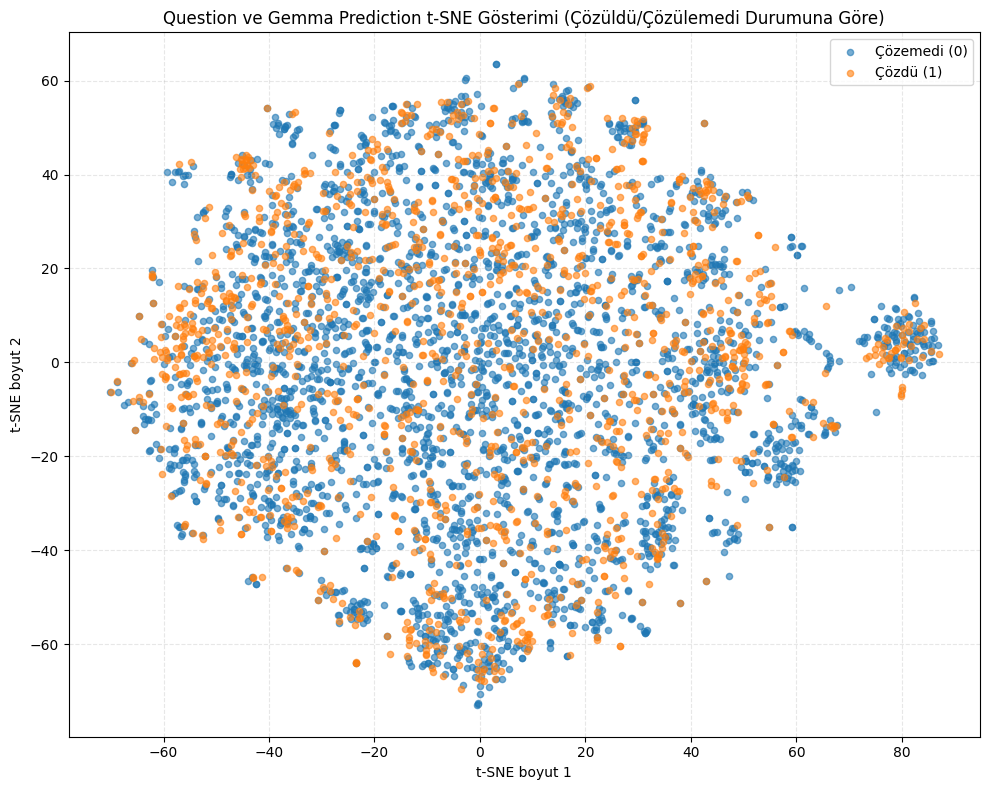
\includegraphics[width=1\linewidth]{q-g.png}
\caption{Sorular embedding'i kullanılarak yapılan Google Gemma tahminleri}
\label{fig}
\end{figure}

\begin{figure}[htbp]
\centering
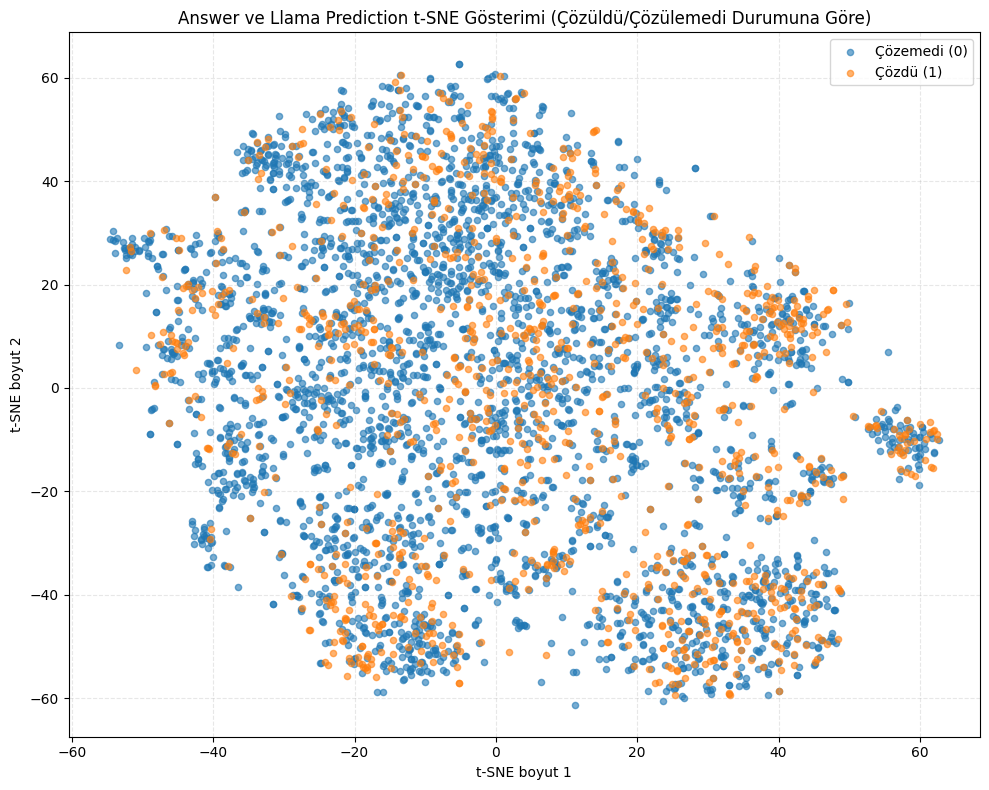
\includegraphics[width=1\linewidth]{a-l.png}
\caption{Cevaplar embedding'i kullanılarak yapılan TR-LLaMa tahminleri}
\label{fig}
\end{figure}

\begin{figure}[htbp]
\centering
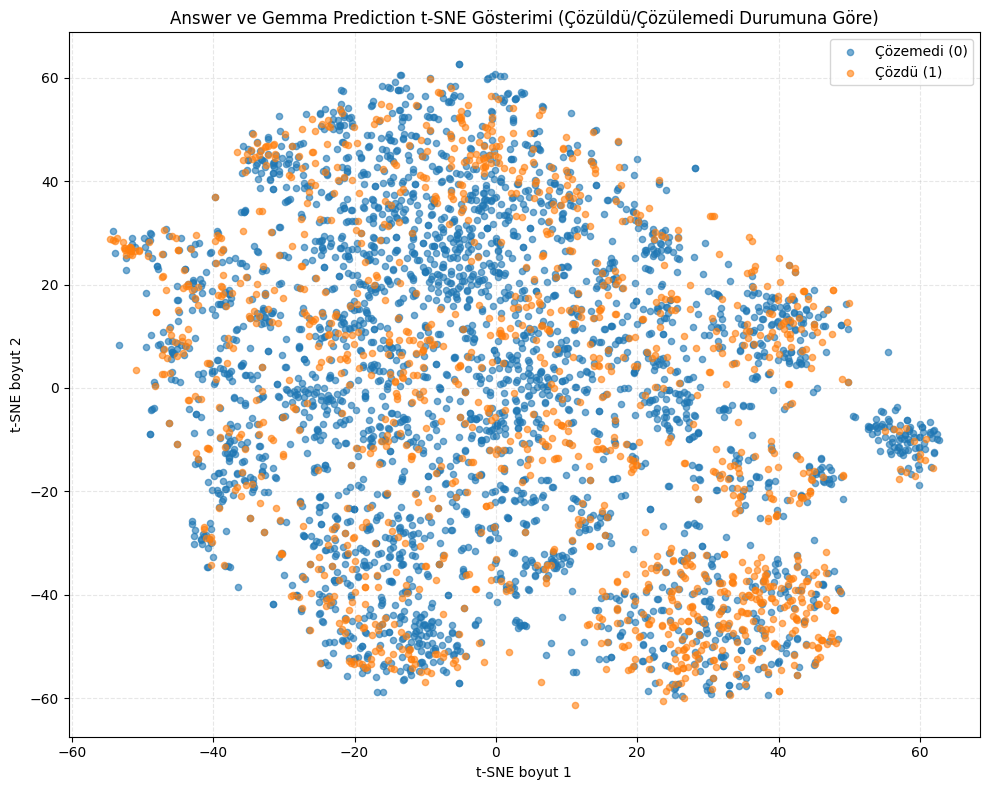
\includegraphics[width=1\linewidth]{a-g.png}
\caption{Cevaplar embedding'i kullanılarak yapılan Google Gemma tahminleri}
\label{fig}
\end{figure}

\begin{figure}[htbp]
\centering
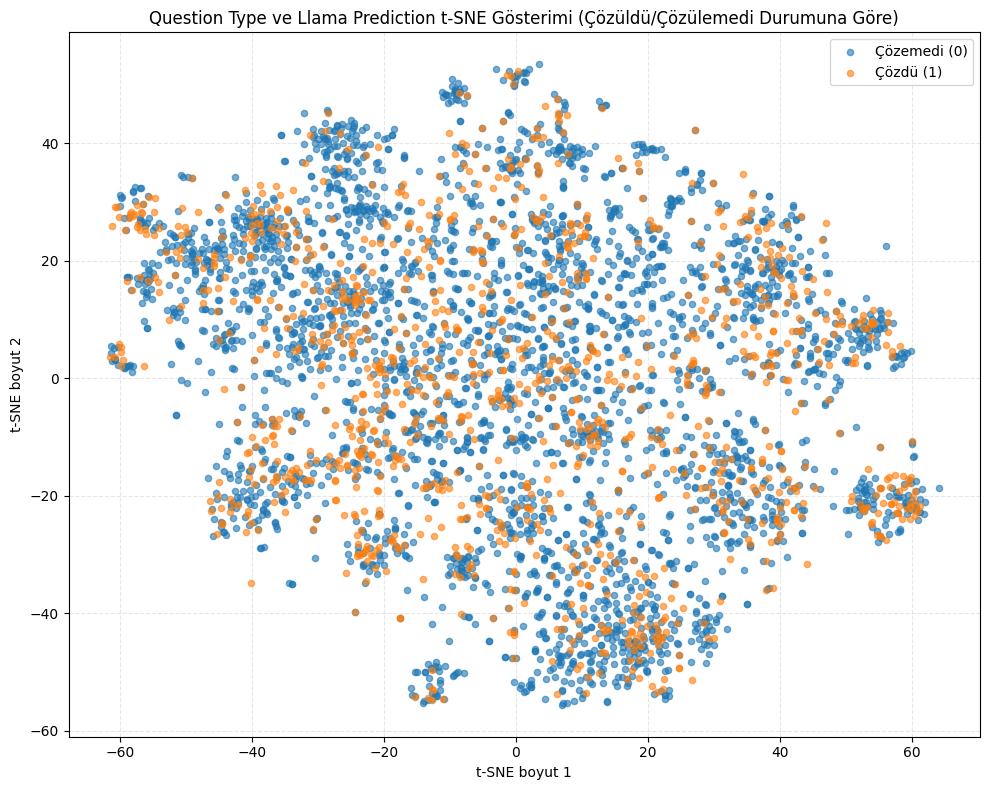
\includegraphics[width=1\linewidth]{qt-l.png}
\caption{Soru tipleri embedding'i kullanılarak yapılan TR-LLaMa tahminleri}
\label{fig}
\end{figure}

\begin{figure}[htbp]
\centering
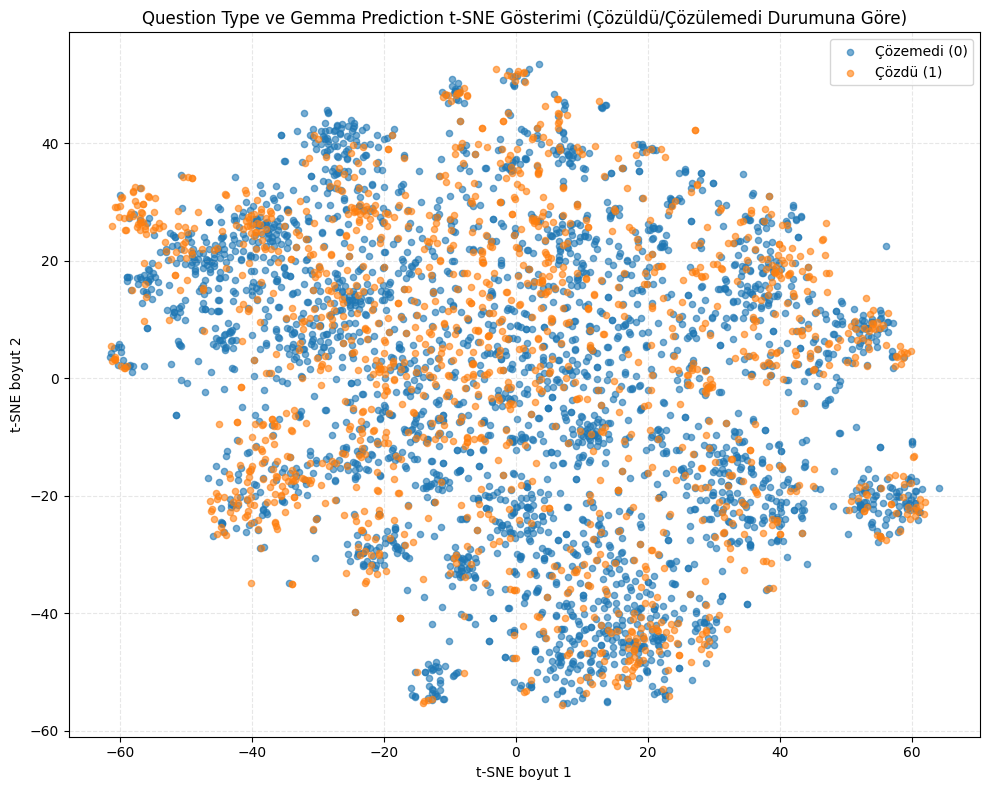
\includegraphics[width=1\linewidth]{qt-g.png}
\caption{Soru tipleri embedding'i kullanılarak yapılan Google Gemma tahminleri}
\label{fig}
\end{figure}

\begin{figure}[htbp]
\centering
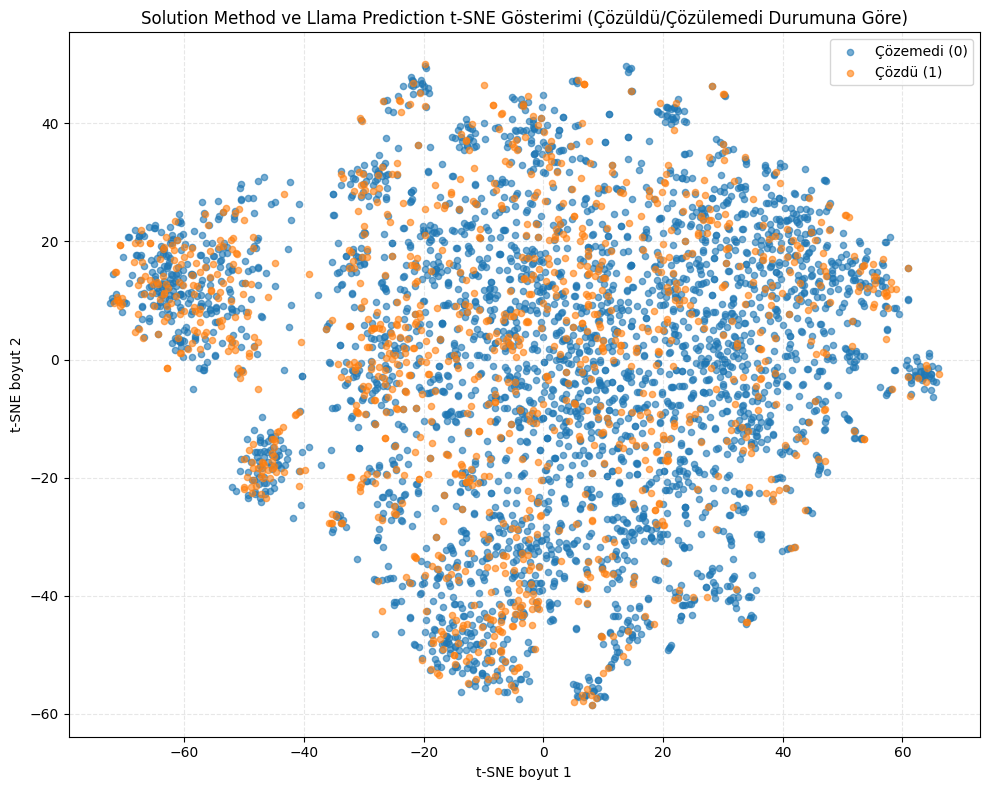
\includegraphics[width=1\linewidth]{sm-l.png}
\caption{Çözüm metotları embedding'i kullanılarak yapılan TR-LLaMa tahminleri}
\label{fig}
\end{figure}

\begin{figure}[htbp]
\centering
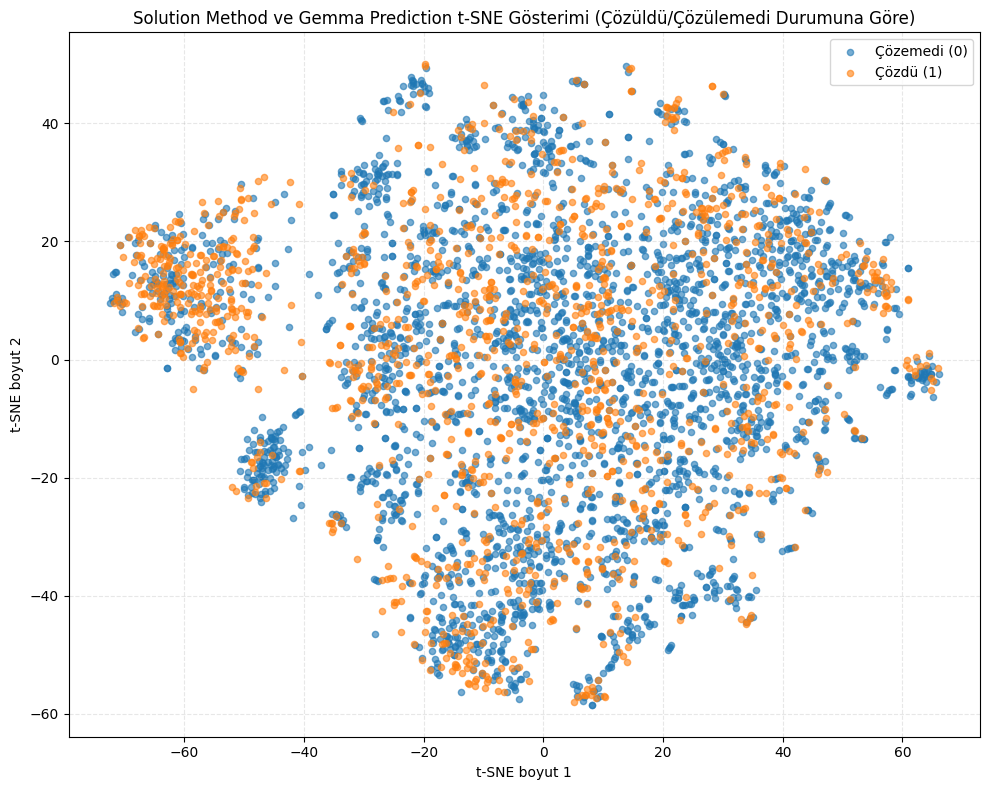
\includegraphics[width=1\linewidth]{sm-g.png}
\caption{Çözüm metotları embedding'i kullanılarak yapılan Google Gemma tahminleri}
\label{fig}
\end{figure}

\section{Sonuç}
Bu çalışmada, GSM8K\_TR veri kümesi üzerinde iki Türkçe LLM'in performansı embedding-tabanlı bir sınıflandırma ve görselleştirme akışıyla değerlendirilmiştir. Llama modeli genel doğrulukta üstünlük sağlarken, Gemma modeli minority örnekleri hatırlama (recall) alanında bir miktar avantaj sunmuştur. Gelecek çalışmalarda veri dengesizliği ve ek öznitelik mühendisliği stratejilerinin performansı nasıl etkilediği araştırılabilir.

\end{document}
